\subsection{Complete spatial profiles and compact summaries}\label{sec:anaheim}
The public Anaheim network has 416 nodes, 914 directed links and 1,406 positive OD demands \citep{tnfrc2024transportation}. Six largest demands change jointly from 0.8 to 1.2 times their published values; other demands remain fixed with endogenous route choices. Ten fixed free-flow shortest paths per OD exclude other zone centroids as intermediate nodes (first through node 39). This calculation uses the existing 41-state attribution columns.
To obtain interpretable region locations without requiring coordinates, define free-flow progress $p(v)=[d_s(v)-d_t(v)+d_s(t)]/[2d_s(t)]$, using shortest distances in the underlying undirected network with the smaller free-flow time on parallel roads --- a network-distance indicator used for ordering the family, not a behavioural travel progress (assignment paths additionally exclude other zone centroids, the progress metric does not). The origin has progress zero and destination progress one. Group tied levels, retain prefixes with two connected induced sides that separate the OD, and orient every region toward the origin. This distance-based family depends on the network and query, before inspecting any attribution. It is a prescribed family, not all connected regions, and it is single-direction: the nested prefixes are totally ordered by progress, so no direction grouping is needed here.

The case asks one transport question: how does the signed crossing-cost
response of the demand change evolve along the origin--destination
direction, and does the variation come mainly from the study traffic's
congestion adjustment or from background rerouting?
Figure~\ref{fig:anaheimprofile} gives the answer for the query with the
largest early--late difference: the account as a function of progress
over the complete family with its delivered four-segment summary, and
the four-part same-state decomposition along the same axis. The
profiles of the remaining five queries stay positive with family ranges
spanning roughly one to one and a half orders of magnitude
(largest-to-smallest account ratios 12.5--36.9); the complete per-query
numbers --- system contributions, unrestricted and family ranges,
region counts and the accounts of the three prespecified positions ---
are collected in Appendix~\ref{app:anaheimsettings}
(Table~\ref{tab:anaheim}), with the early--late mechanism differences
in Table~\ref{tab:anaheimmechanism}.
\begin{figure}[t]\centering
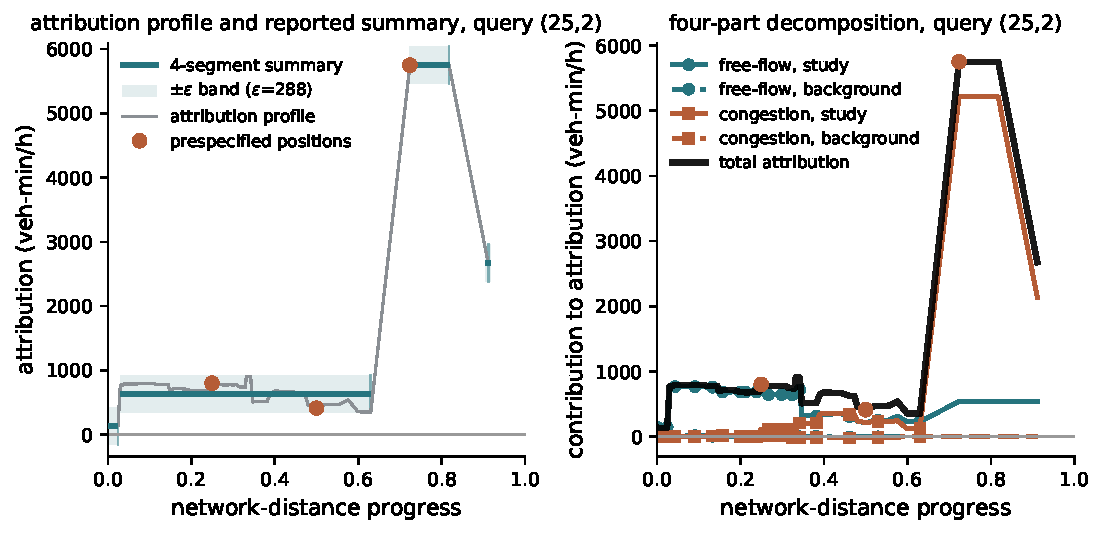
\includegraphics[width=0.99\linewidth]{../figures/fig_v108_anaheim_profile.pdf}
\caption{Anaheim spatial response profile for query $(25,2)$ over the
distance-based family, with its delivered summary. Left: the account
versus free-flow progress along its own OD direction (grey curve); the
four-segment minimum summary at the family tolerance is overlaid
(teal step curve with $\pm\epsilon$ band, $\epsilon=287.6$), and ochre
dots mark the three prespecified positions (nearest admissible gaps to
progress $0.25$, $0.50$, $0.75$). Right: the four-part same-state
decomposition, crossing free-flow and congestion weights with study
and background responses at identical states (teal: free-flow weights,
ochre: congestion weights; solid: study response, dashed: background);
the grey curve is the total account. Components close within
$2\times10^{-12}$ vehicle-minutes per hour.}\label{fig:anaheimprofile}
\end{figure}
Query $(25,2)$ falls from 801.5 at progress $0.250$ to 412.0 at $0.500$
and then rises to the family maximum 5751.2, which holds on the plateau
from progress $0.724$ to $0.818$ before falling back to 2673.1 at
$0.911$. The delivered summary is four segments
(Table~\ref{tab:anaheimsegments}): an origin-side segment near the
family minimum, a long corridor segment covering progress $0.03$--$0.63$
at representative value $630.2$, the congestion plateau at $5751.2$,
and a destination-side position at $2673.1$; every account lies within
$\epsilon=287.6$ of its segment value, the tolerance being $5\%$ of the
family maximum. The decomposition panel locates the mechanism. At the
early position the account is dominated by the free-flow study response
($669.3$ of the total $801.5$, congestion study $111.5$, background
below $11$); at the middle position the two study terms are comparable
($211.5$ free-flow against $212.6$ congestion of the total $412.0$,
background below $11$); at the late position the congestion study term
reaches $5213.7$ while both background terms are below $0.1$ in
absolute value: the rise is congestion adjustment of the study traffic
itself on destination-side links, not background rerouting. The
decomposition is additive at a common equilibrium state and identifies
the contribution of each response--weight component; the summary then
states, with its error bound, where that variation changes.
\begin{table}[t]\centering\footnotesize
\caption{Delivered minimum-segment summaries on Anaheim at the family
tolerance ($5\%$ of the largest account magnitude per query,
Proposition~\ref{prop:segmented}). Segment values are midpoints of the
enclosed account range; every account in a segment lies within the
query's $\epsilon$ of the stated value. Detail for the remaining
queries appears in Appendix~\ref{app:anaheimsettings}.}\label{tab:anaheimsegments}
\setlength{\tabcolsep}{4pt}
\begin{tabular*}{\tblwidth}{@{\extracolsep{\fill}}lrcccc}
\toprule
Query & Regions & Segments & \multicolumn{3}{c}{Segment progress ranges [value]}\\
\cmidrule(lr){4-6}
 & & & \multicolumn{3}{c}{(representative account, vehicle-min/h)}\\
\midrule
$(4,2)$ & 211 & 12 & $[0.04,0.12]$ [3231.5] & $[0.16,0.21]$ [416.4] & $\cdots$ 10 more\\
$(1,2)$ & 83 & 8 & $[0.06,0.18]$ [890.3] & $[0.25,0.37]$ [265.3] & $\cdots$ 6 more\\
$(2,4)$ & 211 & 14 & $[0.04,0.08]$ [1107.9] & $[0.13,0.17]$ [1905.7] & $\cdots$ 12 more\\
$(3,2)$ & 157 & 8 & $[0.05,0.16]$ [908.1] & $[0.23,0.31]$ [298.7] & $\cdots$ 6 more\\
$(25,4)$ & 164 & 13 & $[0.01,0.02]$ [163.1] & $[0.03,0.14]$ [669.1] & $\cdots$ 11 more\\
$(25,2)$ & 84 & 4 & $[0.00,0.02]$ [134.3] & $[0.03,0.63]$ [630.2] & $[0.72,0.82]$ [5751.2], $[0.91,0.91]$ [2673.1]\\
\bottomrule\end{tabular*}\end{table}
The compression is uniform across queries: 83--211 accounts reduce to
4--14 segments ($90.4$--$95.2\%$ compression) with every account within
the stated tolerance by construction, and the summary never changes an
original account --- it is the same computed profile at its coarsest
resolution that meets the tolerance. Aggregation timings and the original construction
costs appear in Appendix~\ref{supp:timing}; the tolerance sensitivity,
including a mixed absolute--relative rule that preserves detail at
small-magnitude positions, appears in Appendix~\ref{supp:tolerance}.
